\chapter{Conclusions}
\label{conclusions}

% **************************** Define Graphics Path **************************

\graphicspath{{Chapter6/Figs/}}

While this thesis explores a number of core computer vision problems --- scene understanding, localisation, stereo and motion --- we can observe some general conclusions. 

Firstly, end-to-end deep learning has emerged as the prevailing paradigm for modelling computer vision problems. For all of the tasks in this thesis, end-to-end learning is able to outperform hand-engineered approaches. It reduces engineering effort and performs very well by optimising the model with respect to the end goal.

In general, we find using representations of geometry improves the representational power of vision models. It improves performance of models by simplifying the learning task and allows models to learn from unsupervised learning, greatly reducing the dependence on labelled training data.

Finally, probabilistic or Bayesian deep learning is a practical framework for quantifying model uncertainty for vision tasks. We showed that it is important to model uncertainty for safety-critical applications, to understand examples which are different from training data, and small datasets where the training data is sparse.

\section{Findings and Limitations}

We briefly summarise the findings and limitations of each chapter in this thesis.

\cref{scene_understanding} presented SegNet, a deep learning framework for dense pixel-wise output. We showed its efficacy for semantic segmentation, instance segmentation and depth regression. We compared different techniques for upsampling and show the advantage of learning filters and using information from the encoder. However, the model often fails to capture objects at different scales and reason within the context of the whole image. We derived a practical Bayesian deep learning formulation to capture aleatoric and epistemic uncertainty. We demonstrate how to use uncertainty to weight multiple tasks to jointly learn semantics and geometry.

\cref{localisation} introduces PoseNet, a convolutional neural network for camera pose regression. We show that it is faster and more scalable than traditional structure from motion methods for localisation. While it is more robust to challenging appearance changes, it cannot produce the same level of fine-grained accuracy as classical geometry. However, explicitly using geometric and reprojection error loss functions can improve results. Modelling uncertainty is useful to determine metric relocalisation error and estimate loop closure. Although, this method is only capable of relocalisation, and does not address the problem of online-learning or localisation over video sequences.

\cref{stereo} shows an end-to-end deep learning architecture for stereo disparity regression. We show it can outperform prior hand-engineered models while being significantly more accurate. However, the model forms the full cost volume and is not real-time. Further work is needed, perhaps with hierarchical models, for efficient inference. Although, we find we can use geometry for unsupervised learning by learning from photometric reprojection error. Finally, we show uncertainty is useful to attenuate noisy training labels and to combine semi-supervised and unsupervised learning. However, our probabilistic model assumes uni-modal Gaussian distributions which is not always accurate.

\cref{motion} introduces deep learning models which can learn video scene understanding over long video sequences. We show the benefits of explicitly modelling depth and motion. In order to train models over video we find there are a number of important factors to consider. We introduce temporal loss functions and show how to jointly learn semantic segmentation with supervised learning, and depth and optical flow with unsupervised learning.

\section{Applications}

This work has an array of practical applications. \cref{ch6:applications} shows technology which directly use the ideas and software developed in this thesis. We briefly describe three general application areas of this work.

\begin{figure}[t]
\center
    \begin{subfigure}[t]{0.32\textwidth}
        \centering
          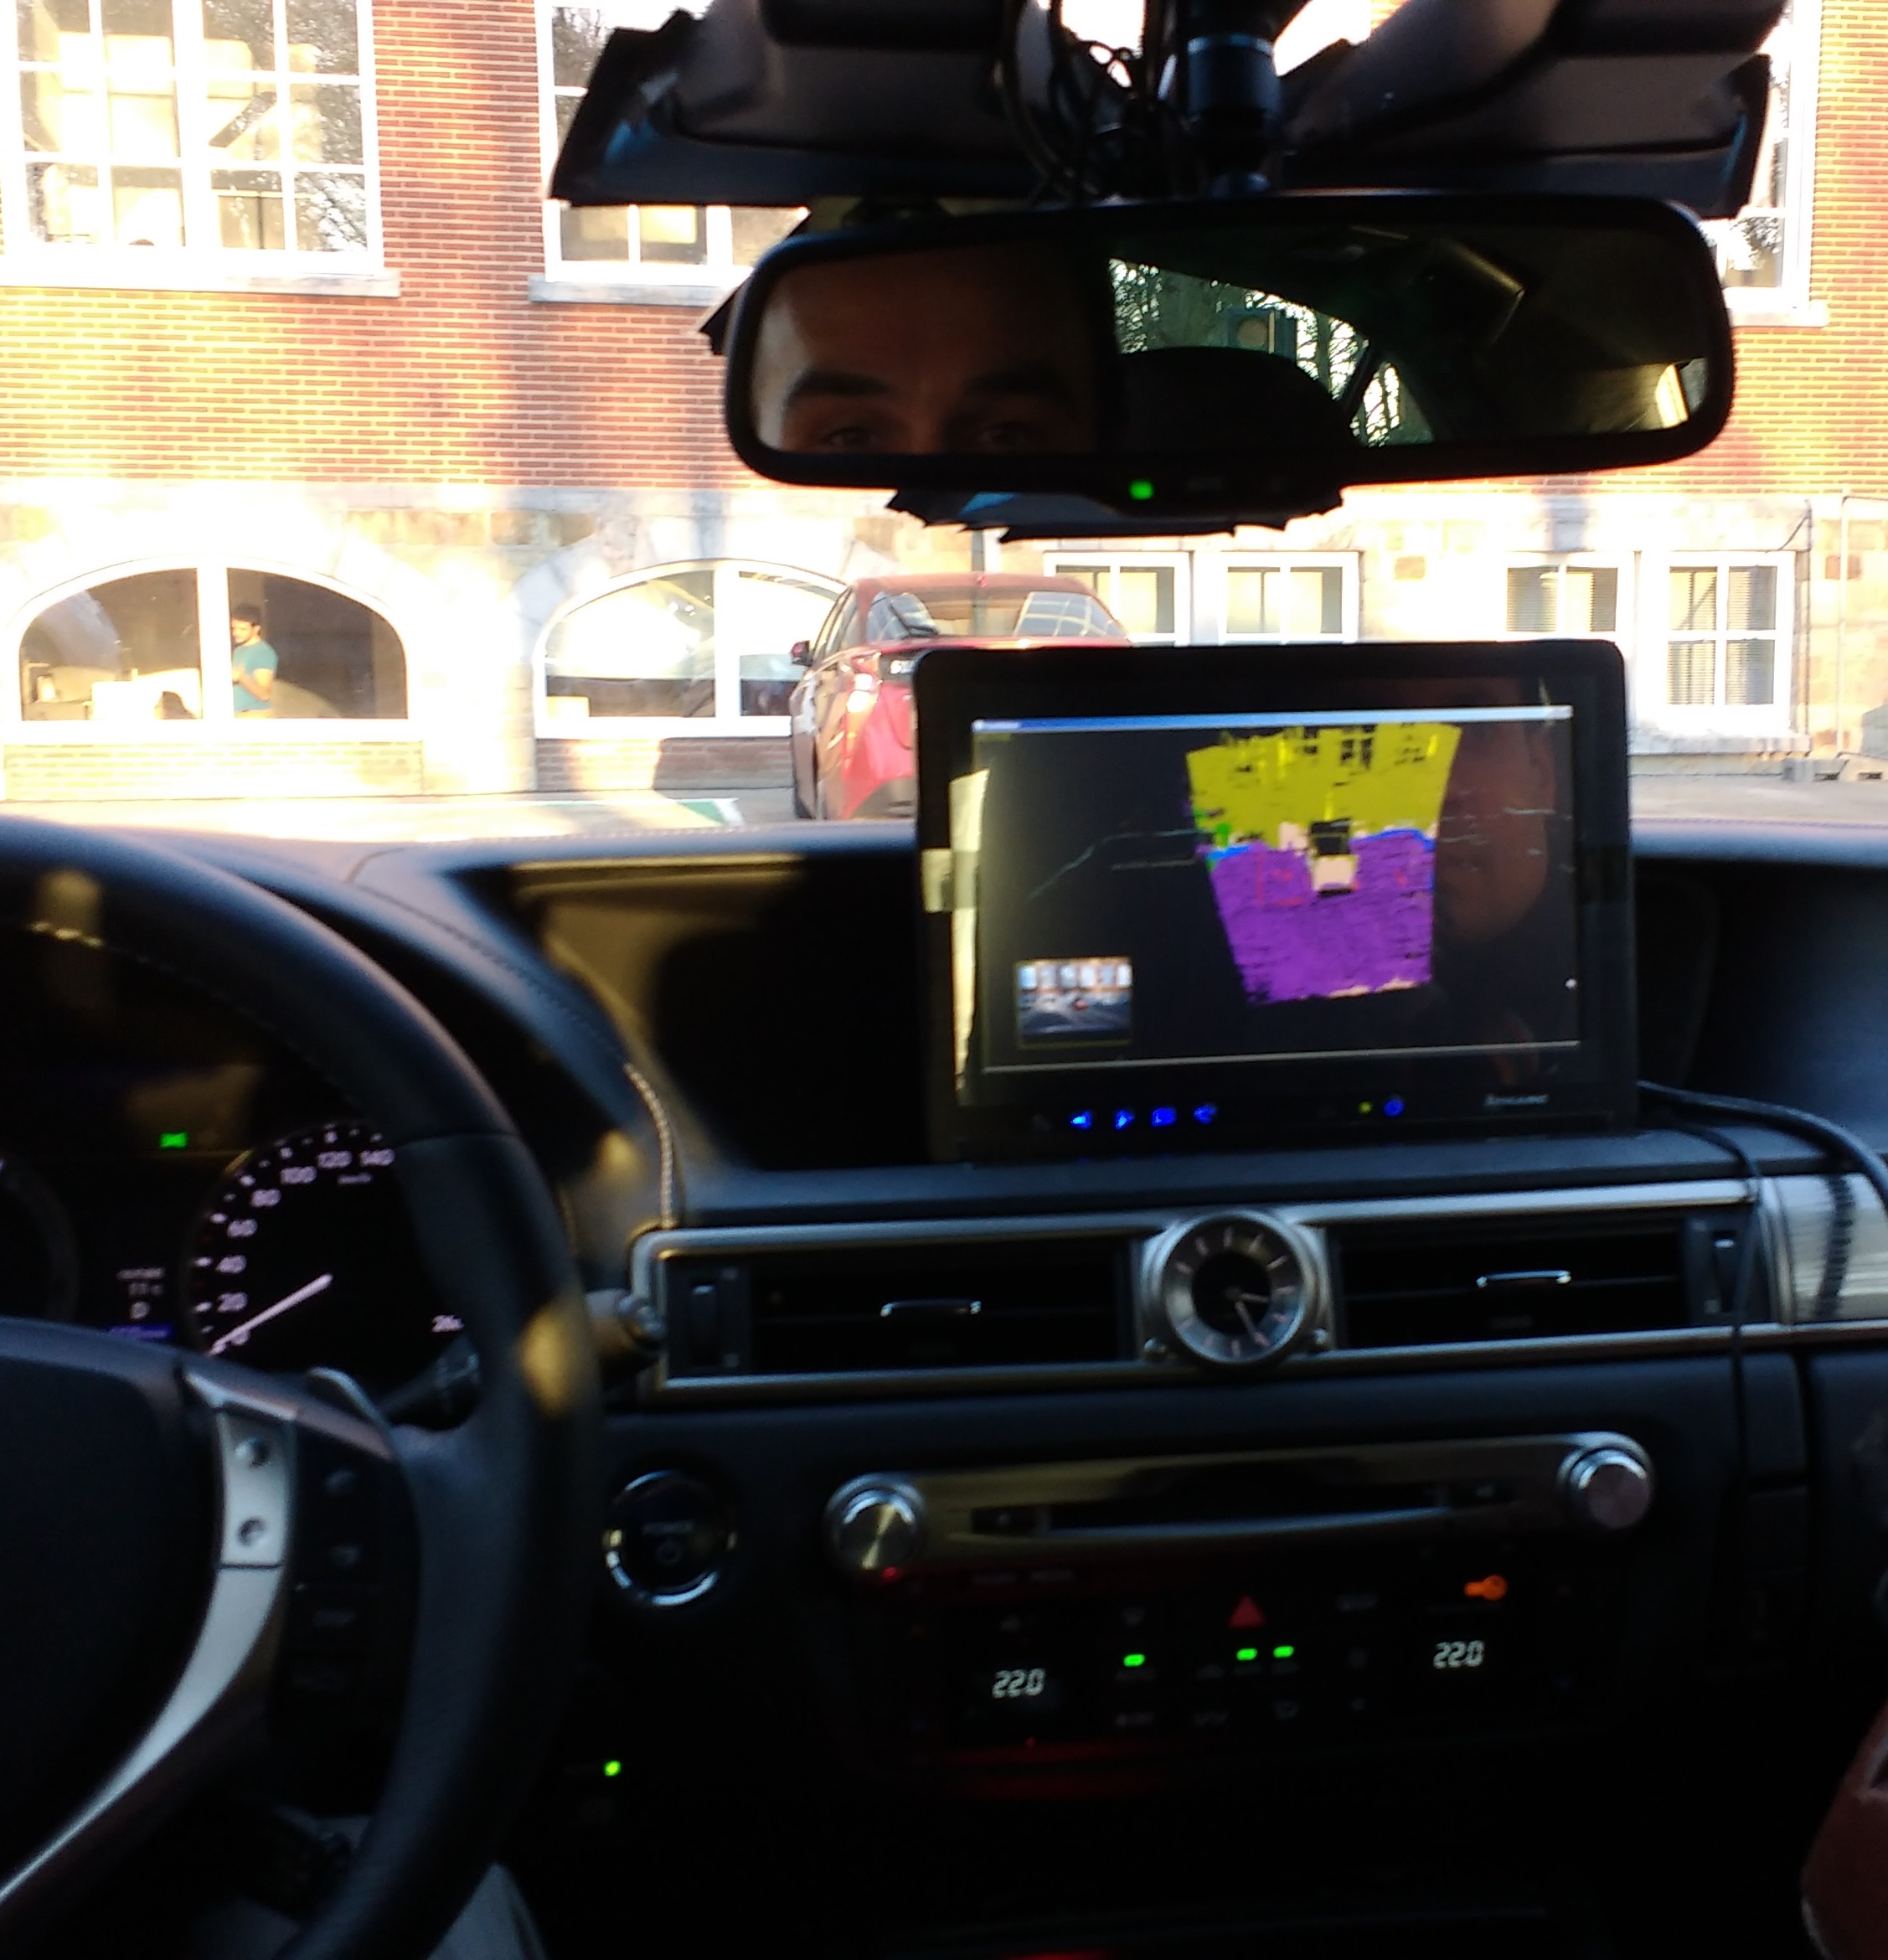
\includegraphics[height=5cm]{toyota.jpg}
        \caption{Autonomous vehicles and self-driving cars.}
    \end{subfigure}
    \begin{subfigure}[t]{0.32\textwidth}
        \centering
          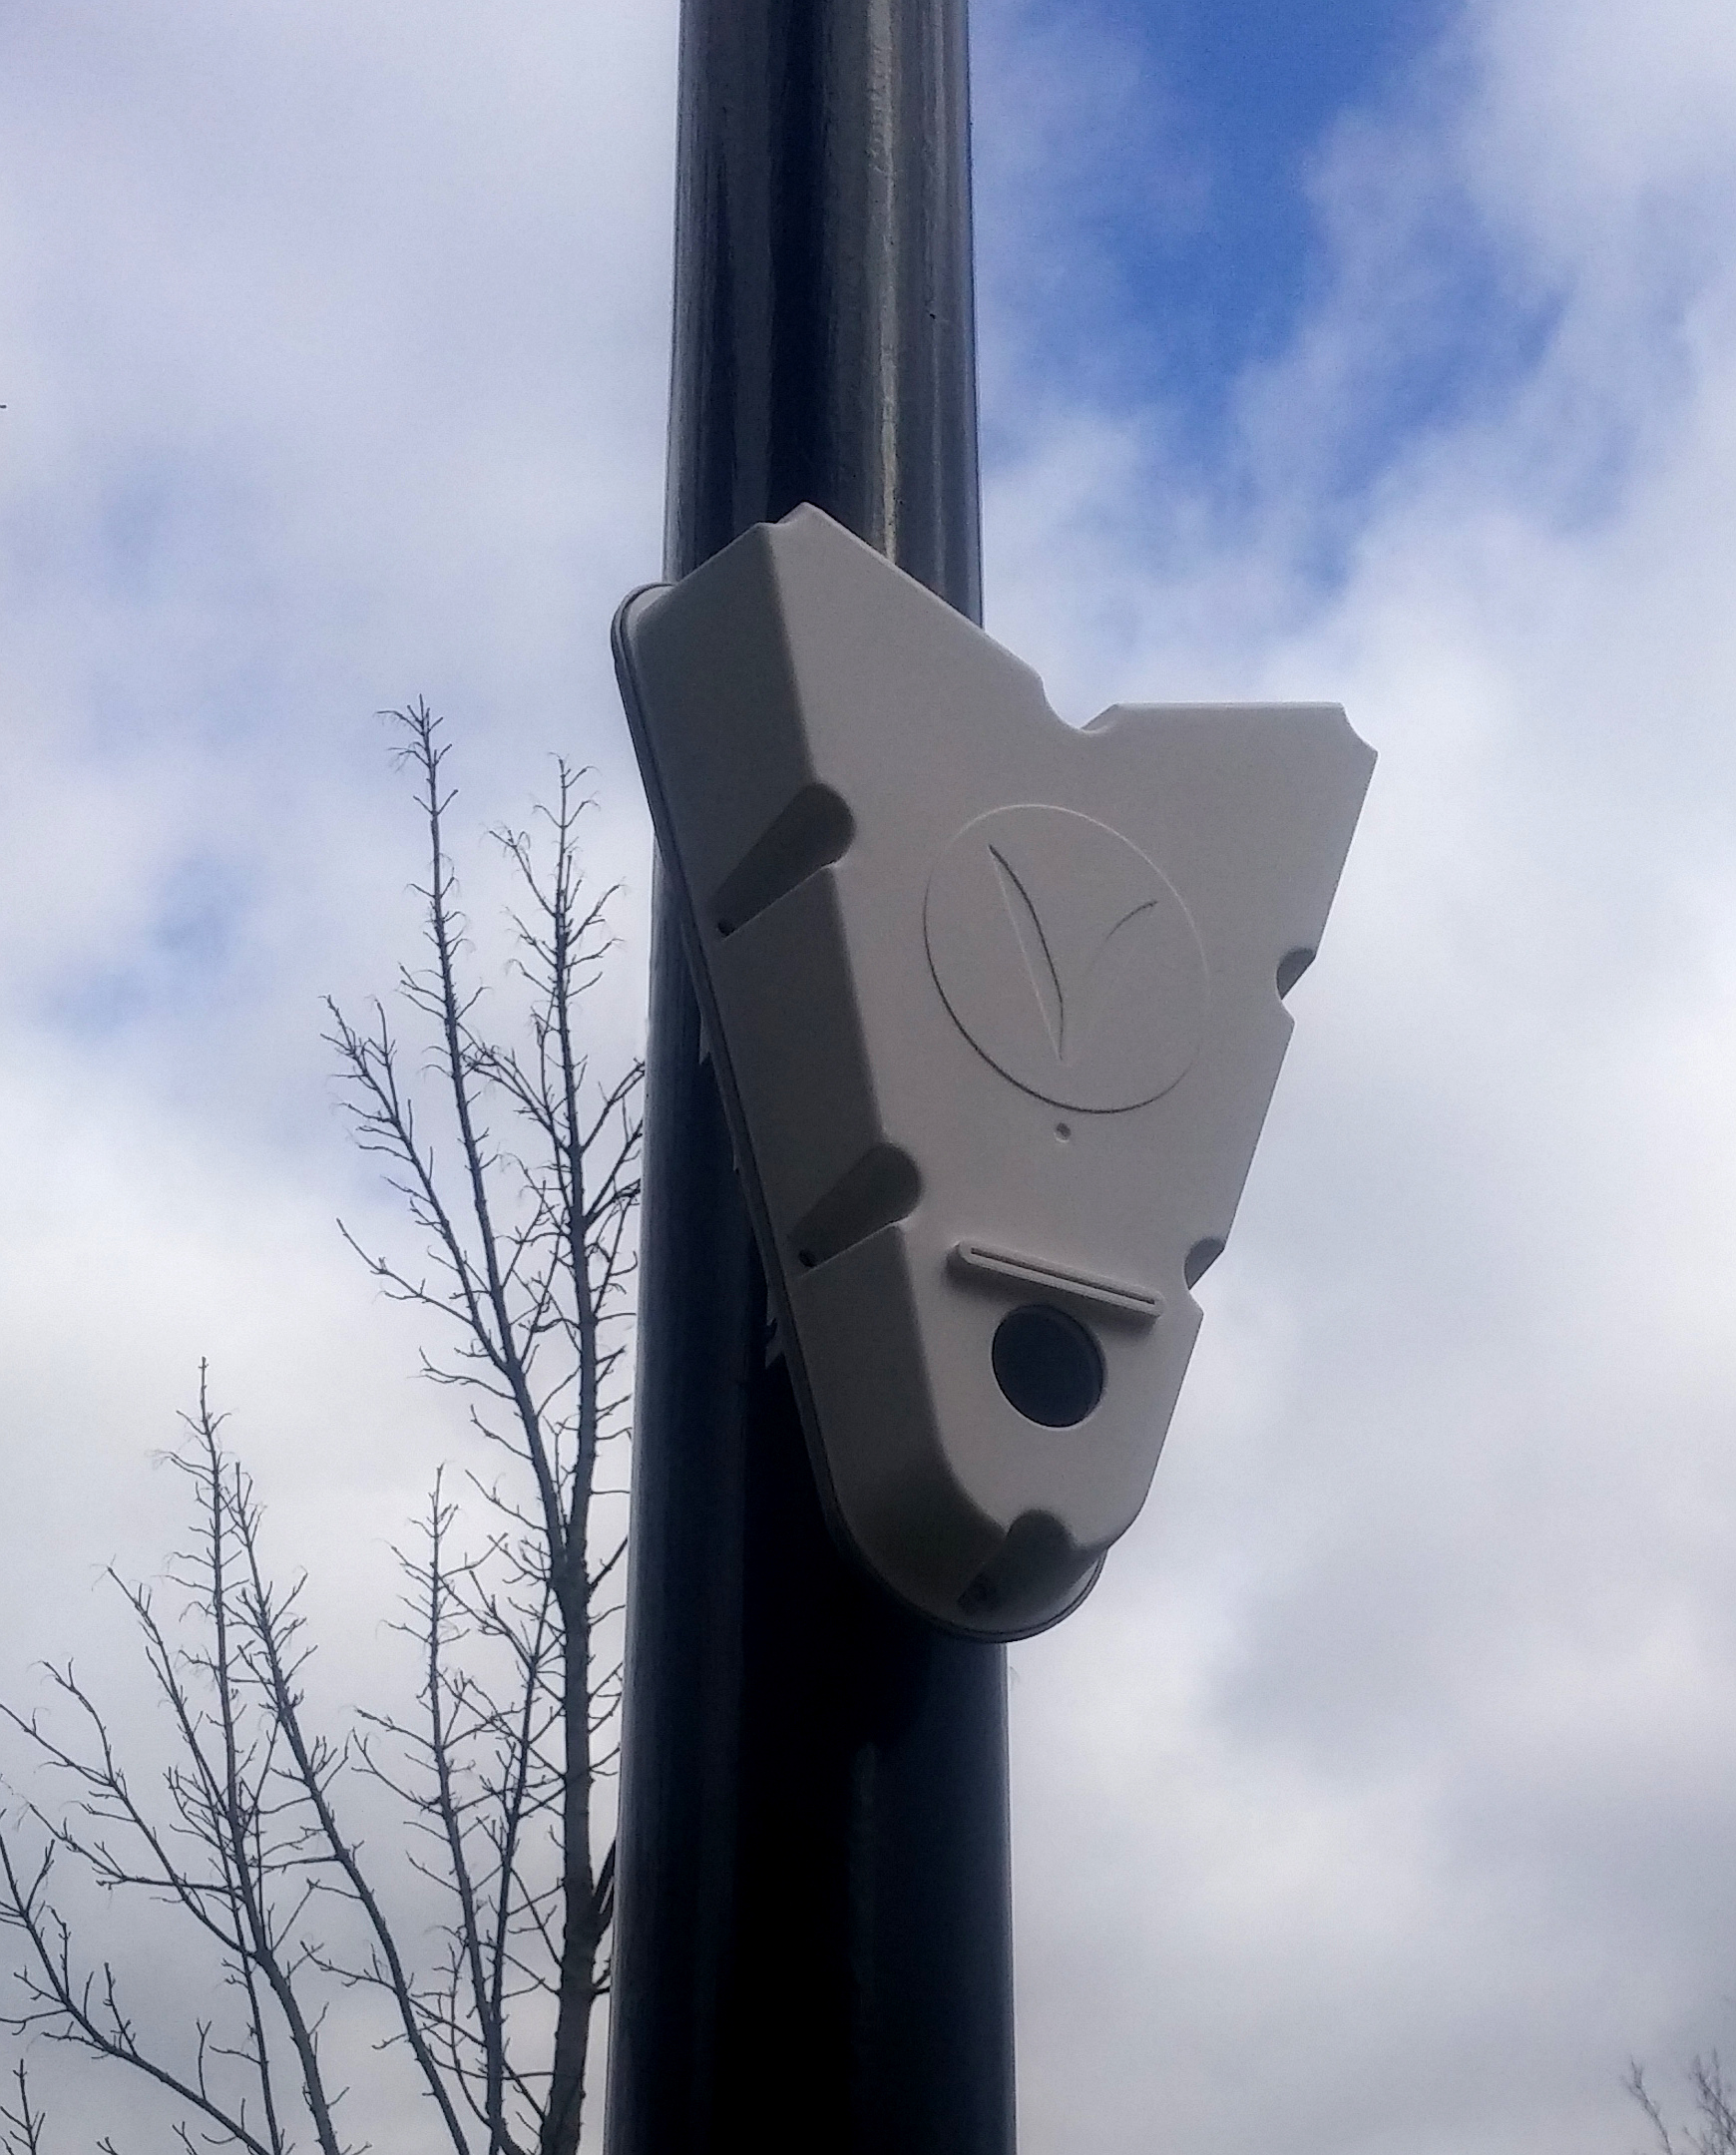
\includegraphics[height=5cm]{vivacity.jpg}
        \caption{Smart cities and intelligent surveillance.}
    \end{subfigure}
    \begin{subfigure}[t]{0.32\textwidth}
        \centering
          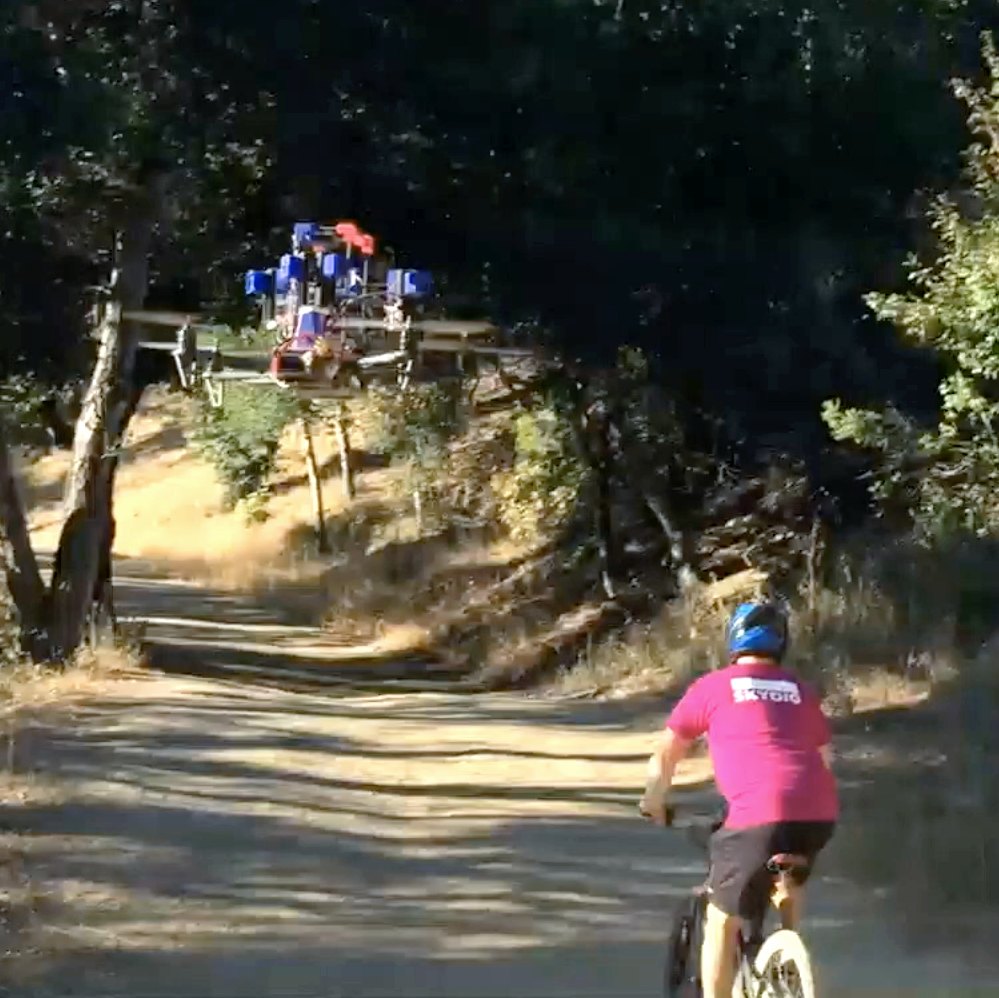
\includegraphics[height=5cm]{skydio.png}
        \caption{Autonomous unmanned aerial vehicles.}
    \end{subfigure}%
\caption[Applications of technology in this thesis]{\textbf{Applications of the technology developed in this thesis.} Algorithms and software which was written as part of this thesis are inside many of today's products, including these three examples. (a) shows a prototype autonomous vehicle running SegNet for real-time scene understanding. (b) shows a smart-city sensor by Vivacity \citep{vivacity} running software from this thesis. (c) shows a prototype drone from Skydio \citep{skydio} using algorithms and software from \cref{scene_understanding} to understand scene semantics and geometry.}
\label{ch6:applications}
\end{figure} 

\subsection{Robotics}
Understanding the scene’s geometry and semantics is a fundamental task for autonomous robots. This provides information of the free space to avoid obstacles and where objects. This enables robots to interact intelligently with the world. The ideas from \cref{scene_understanding} and \cref{motion} allow us to build such a system with end-to-end deep learning.

Cameras are attractive sensors because they are cheap, they are passive and require low-power. The algorithms presented in this thesis can operate in real-time on robotic platforms with relatively cheap cameras and computation. For example, on autonomous vehicles, self-driving cars, drones and domestic robots \citep{kendall2014board,mcallister2017av_bdl}.

The challenges for this application are about obtaining sufficient and robust performance within a real-time computational budget. The ideas about using geometry will be beneficial here. It is also critical these systems understand their uncertainty to make safe policy decisions based on well-founded information. Therefore, the ideas presented on modelling uncertainty are also highly useful.

\subsection{Smart-Cities and Surveillance}
In addition to robotics, computer vision algorithms are useful to understand scenes from fixed cameras. One can imagine smart city infrastructure, or internet-of-things (IOT) devices which would benefit from visual scene understanding. Semantic and instance video segmentation are important technologies. These could have applications for security monitoring, collecting behaviour statistics and providing analytics of the world in real-time.

\subsection{Medical Imaging}
Computer vision is proving successful in advanced diagnosis of medical images \citep{ronneberger2015u}. However, obtaining training data is difficult and it is often biased against rare conditions and diseases. Therefore, it is important to account for uncertainty when making a diagnosis, with many of the ideas in this thesis very useful for this task. Medical imaging also often involves 3-D data with images obtained in voxels. Geometry may assist deep neural networks to learn more efficiently and be more effective in this domain.

\subsection{Augmented Reality}
Augmented reality provides an improved interface to data by overlaying it on the world we see. For example, wearable technology like glasses can overlay information such as advertising on shop façades, directions on the street or Pokémon to play with.

Augmented reality systems require accurate depth and semantic scene understanding. Global camera pose estimation is also of interest to overlay virtual worlds. Ideas from \cref{localisation} for localisation and other ideas in this thesis about learning geometry can be used. Applications include entertainment, education or improving the accessibility of information.



\section{Future Work}

To conclude this thesis, there are many aspects of important future work which we would like to highlight. As is typical with any research, this thesis raises more questions than answers. Improvements to the individual algorithms have been discussed within the body of this work. However, at a high level we would like to highlight the following themes for future research which are particularly exciting.

\subsection{Learning Geometry with Memory}
A great challenge in artificial intelligence research is learning representations with memory \citep{graves2014neural}. Today, this is typically approached in language and sequence modelling fields \citep{weston2014memory}. However, we believe geometry offers an excellent setting to learn memory, because we can learn geometry with unsupervised learning. An example, is the problem of simultaneous localisation and mapping \citep{durrant2006simultaneous}, where a model must learn to build a map while experiencing a world. This is a task the human brain performs very well \citep{moser2008place,o1978hippocampus}. Learning this with a computer vision system provides an excellent setting to challenge the best geometry and memory networks.

\subsection{More Flexible Uncertainty Distributions}
This thesis has argued that understanding uncertainty is essential for safe computer vision systems. However, Bayesian deep learning often underestimates uncertainty (\cref{scene_understanding}). It is important we improve the calibration of this uncertainty. In this thesis, one assumption all probabilistic models made was that the probability distribution is Gaussian. In reality, this may not be a valid claim. One important area of future research is learning more flexible distributions and multi-modal distributions which can represent the real-world more effectively. For example, multi-modal predictions are particularly important for predicting the future, which we describe next.

\subsection{Predicting the Future}
This thesis has addressed algorithms for understanding semantics and geometry from both individual images and video sequences. However, another large problem which has not been mentioned so far is, \textit{what is going to happen next?} Predicting scene dynamics is an important problem to solve in computer vision, especially for applications in robotics. While there is some initial work in this area \citep{luc2017predicting}, this problem would benefit from the three themes of this thesis; end-to-end deep learning, geometry and uncertainty.

\subsection{Learning to Act}
Finally, the purpose of a brain is for movement \citep{wolpert2000computational}. Therefore, an interesting question is what is the point of learning these representations of semantics, motion and geometry? Ultimately, these algorithms are useful to learn representations for visuomotor control (systems that reason from sensory input to control output). Today, most visuomotor algorithms are naive and do not consider geometry and uncertainty \citep{levine2016end}. Benefits could be observed from leveraging the ideas in this thesis about geometry and uncertainty.
